% ------------------------------------------------------------------------------
% Este fichero es parte de la plantilla LaTeX para la realización de Proyectos
% Final de Grado, protegido bajo los términos de la licencia GFDL.
% Para más información, la licencia completa viene incluida en el
% fichero fdl-1.3.tex

% Copyright (C) 2012 SPI-FM. Universidad de Cádiz
% ------------------------------------------------------------------------------

Este capítulo trata sobre todos los aspectos relacionados con la implementación del sistema en código, haciendo uso de un determinado entorno tecnológico.

\section{Entorno de Construcción}
%En esta sección se debe indicar el marco tecnológico utilizado para la construcción del sistema: entorno de desarrollo (IDE), lenguaje de programación, herramientas de ayuda a la construcción y despliegue, control de versiones, repositorio de componentes, integración contínua, etc.

El framework empleado en la creación de esta página web es \textit{\textbf{Grails}}, un framework para aplicaciones web libre desarrollado sobre el lenguaje de programación \textit{\textbf{Groovy}} (el cual a su vez se basa en \textit{\textbf{Java}}). Groovy posee una sintaxis muy parecida a \textit{Java}, comparte el mismo modelo de objetos, de hilos y de seguridad, además, puede acceder directamente a todas las API existentes en \textit{Java}. Esta relación entre ambos lenguajes, ha permitido que algunas partes del desarrollo se haya empleado tanto \textit{Java} como \textit{Groovy}.\\

Para emplear estos lenguajes en el desarrollo, se emplea el IDE \textit{\textbf{Grails Tool Suite}}, un entorno de trabajo donde podemos aplicar el paradigma \textbf{Modelo Vista Controlador} (MVC).\\

\textit{Grails Tool Suite} es un IDE altamente productivo que sigue paradigmas como convención sobre configuración o no te repitas (DRY) proporcionando un entorno de desarrollo estandarizado y ocultando gran parte de los detalles de configuración al programador.\\

Una de las ventajas que proporciona este tipo de proyectos, es que podemos instalar dependencias y \textit{plugins} que nos permitan instalar utilidades a nuestro proyecto Grails para ser empleadas directamente sobre el código y aplicar el paradigma DRY que se ha explicado anteriormente. Algunos de ellos son:

\begin{itemize}
	\item \textit{tomcat} Para instalar el contenedor de Java Tomcat.
	\item \textit{jquery} Para instalar JQuery en el proyecto.
	\item \textit{spring-security-core} Para realizar la securización de la aplicación web.
	\item \textit{executor} Para realizar tareas en segundo plano.
	\item \textit{apache.poi} Para la creación de documentos word, excel o pdf.
	\item \textit{mysql-connector-java} Para permitir la conexión de la aplicación con MySQL.
\end{itemize}

Todo el código de la aplicación se encuentra ubicado en un espacio de trabajo de Assembla cuya dirección es \url{https://app.assembla.com/spaces/systematic-literature-review/} que puede ser descargado en un equipo por Subversion (SVN). En este espacio de trabajo se ha insertado además todo el contenido de la memoria así como recursos necesarios que puedan ser de utilidad para este trabajo.

\section{Código Fuente}
%Organización del código fuente, describiendo la utilidad de los diferentes ficheros y su distribución en paquetes o directorios. Asimismo, se incluirá algún extracto significativo de código fuente que sea de interés para ilustrar algún algoritmo o funcionalidad específica del sistema.

En la figura \ref{fig:estruc-grails} podemos ver la estructura de directorios que tiene este proyecto Grails.\\

\begin{figure}[!hpt]
	\begin{center} 
		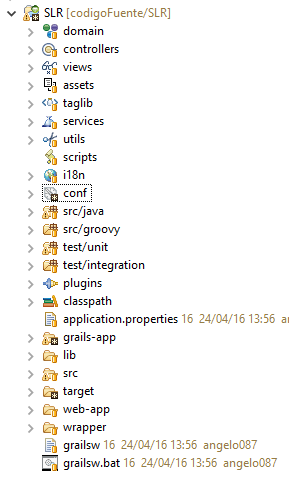
\includegraphics[scale=0.6]{estructura-grails-project.png}
		\caption{Estructura Proyecto Grails}
		\label{fig:estruc-grails}
	\end{center}
\end{figure}

\begin{itemize}
	\item \textbf{conf} Archivos de configuracion
	\item \textbf{controllers} Controladores
	\item \textbf{domain} Entidades
	\item \textbf{i18n} messages bundles
	\item \textbf{services} Servicios
	\item \textbf{taglib} Libreria de etiquetas
	\item \textbf{util} Clases de utilidad
	\item \textbf{views} Vistas
	\item \textbf{layouts} Layouts SiteMesh
	\item \textbf{lib}
	\item \textbf{scripts}
	\item \textbf{src}
	
	\begin{itemize}
		\item \textbf{groovy} Otras clases Groovy
		\item \textbf{java} Otras clases Java
	\end{itemize}
	
	\item \textbf{test} Casos de prueba
	\item \textbf{web-app} Raiz de la aplicacion web
\end{itemize}

Para almacenar todo el código del proyecto en el repositorio assembla, se ha instalado un plugin para el IDE Grails Tool Suite denominado \textit{Subclipse} con el que rápidamente podemos subir todas las modificaciones y ver el histórico de cambios con respecto a otras versiones del código.\\

Como ejemplo de código se va a describir la funcionalidad de crear una búsqueda en una revisión sistemática de la literatura. Primeramente, debemos tener una clase que representa la entidad Search dentro de la carpeta \textit{domain} a la que hemos denominado \textit{Search.groovy} tal y como podemos ver en la \ref{fig:impl-domain}. En ella, podemos destacar la relación con otras clases y los atributos de la clase como una clase de Java.\\

\begin{figure}[!hpt]
	\begin{center} 
		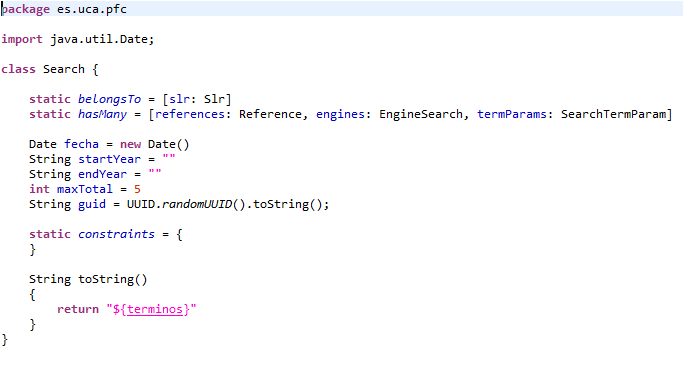
\includegraphics[scale=0.7]{impl-domain.png}
		\caption{Dominio clase Search}
		\label{fig:impl-domain}
	\end{center}
\end{figure}

Cuando el usuario desee crear una búsqueda, elegirá la acción de crear una búsqueda a través de un botón. El controlador será el encargado de recoger esta acción propuesta por el usuario, tratará la información correspondiente y redirigirá a la vista correspondiente. Este controlador se encuentra dentro de la carpeta \textit{controller}. La clase resultante es \textit{SearchController.groovy} tal y como podemos ver en la figura \ref{fig:impl-controller}. En el controlador se recoge todas las acciones que el usuario desee realizar con respecto a una búsqueda. En nuestro caso, comprobará que la búsqueda tenga una revisión sistemática asignada o cargar la lista de motores de búsquedas que el usuario puede emplear entre otras tareas.\\

\begin{figure}[!hpt]
	\begin{center} 
		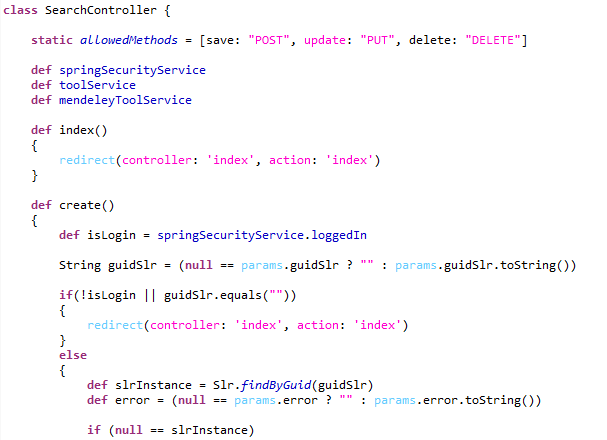
\includegraphics[scale=0.7]{impl-controller.png}
		\caption{Controlador clase Search}
		\label{fig:impl-controller}
	\end{center}
\end{figure}

Una vez que el controlador acaba sus tareas y comprobaciones, redirigirá la acción a una vista donde mostraremos el formulario con el que el usuario podrá ingresar los parámetros de búsqueda que estime necesario. Grails posee una carpeta denominada \textit{view} donde se encuentran organizadas todas las vistas por controladores y acciones. En nuestro caso, habrá una vista denominada \textit{create.gsp} dentro de la carpeta \textit{search}, que a su vez estará dentro de la carpeta \textit{view}. Esta vista (ver figura \ref{fig:impl-view}) posee todo el contenido HTML y etiquetas de grails que muestra el formulario que permite al usuario crear una búsqueda dentro de la aplicación web.\\

\begin{figure}[!hpt]
	\begin{center} 
		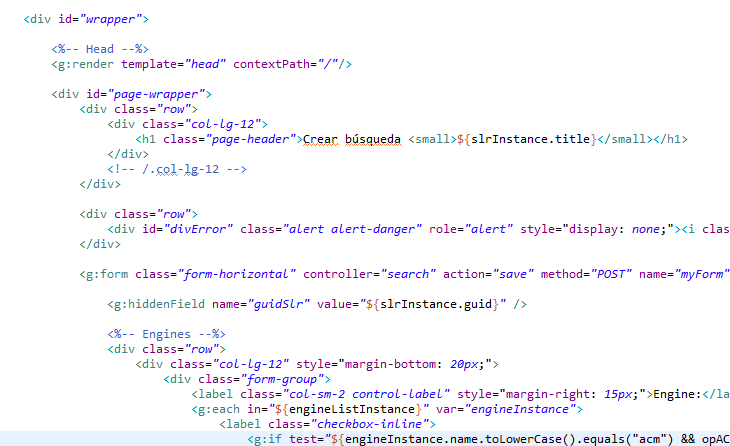
\includegraphics[scale=0.7]{impl-view.png}
		\caption{Vista clase Search}
		\label{fig:impl-view}
	\end{center}
\end{figure}

Posteriormente, el usuario rellena el formulario y elegirá la opción de realizar la búsqueda. Por tanto, volvemos al mismo mecanismo que hemos explicado anteriormente pero con diferentes acciones. En este caso, volvemos al controlador de la búsqueda donde tendrá la acción \textit{save} y ésta se encarga de comprobar que los parámetros introducidos son correctos. En caso de ser así, redigirá la acción a la lista de búsquedas ya realizadas notificando con un mensaje que la búsqueda está en proceso. En caso contrario, redigirá la salida a la pantalla de creación de búsquedas con un mensaje de error.\\

Por último, dentro de cualquier controlador, podremos implementar unas clases o servicios que se encargan de la implementación de algunas de las funcionalidades. Ya en \ref{fig:impl-controller} pudimos ver que hay un servicio definido denominado \textit{springSecurityService}, el cuál, se encarga de la gestión de usuarios. Este servicio es creado gracias a un plugin que se ha instalado, pero podemos crear nuestros propios servicios. En nuestro caso, se ha decidido crear un servicio que realice las búsquedas para la conexión con Mendeley y realice las búsquedas en segundo plano al que hemos determinado \textit{mendeleyToolService} y que también podemos ver definido en \ref{fig:impl-controller}. La implementación de este servicio se encuentra dentro de la carpeta \textit{service} bajo el nombre \textit{MendeleyToolService.groovy} tal y como podemos ver en la figura \ref{fig:impl-service} y se realizaría bajo el método \textit{insertSearchsBackground} como una función típica de Java.

\begin{figure}[!hpt]
	\begin{center} 
		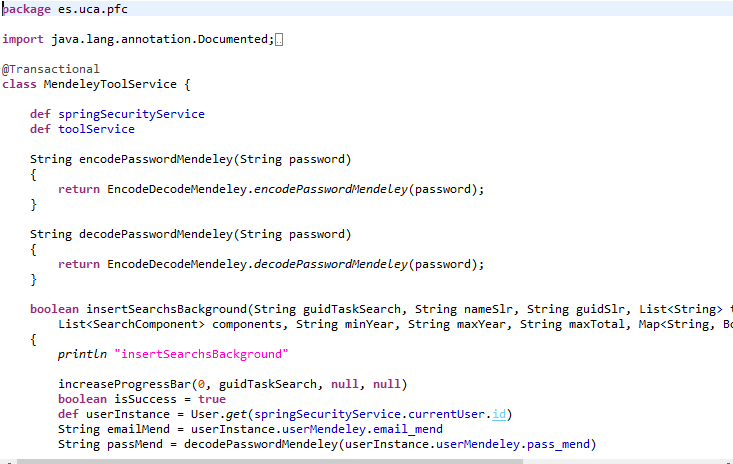
\includegraphics[scale=0.7]{impl-service.png}
		\caption{Vista clase Search}
		\label{fig:impl-service}
	\end{center}
\end{figure}

\section{Scripts de Base de datos}
Organización del código fuente, describiendo la utilidad de los diferentes ficheros y su distribución en paquetes o directorios. Asimismo, se incluirá el script de algún disparador o un procedimiento almacenado, que sea de interés para ilustrar algún aspecto concreto de la gestión de la base de datos.
